\beamertxt{\pagebreak}
\section{TID angewandt 1}
\label{sec:TID_angewandt1}
Betrachten Sie die unten skizzierte Ausgangssituation: Es sind Blöcke mit einer Größe von 48~Byte (ein Byte ist hier jeweils durch ein Kästchen repräsentiert) gegeben. Block~0 enthält zum Ausgangszeitpunkt genau 2 Sätze: TID(0, 0) mit der Länge 7 und TID(0, 1) mit der Länge 17.

Gehen Sie von einem stark vereinfachten TID-Konzept aus: Legen Sie lediglich die Nutzdaten der Sätze selbst, bei einem Überlauf die neue TID eines Satzes und die Indexeinträge für die Sätze in den Blöcken ab. Zusätzliche Informationen, wie den normalerweise üblichen TID-Header und Längeninformationen zu jedem Satz, können Sie vernachlässigen. Nehmen Sie an, dass für einen Indexeintrag genau 1~Byte, und für eine TID genau 2~Byte Speicherplatz benötigt werden. Darüber hinaus müssen Sie sich auch keine Gedanken darüber machen, wie erkannt wird, ob es sich bei den abgelegten Daten um Nutzdaten, eine TID oder einen Indexeintrag handelt.

\begin{beamerText}
\pagebreak

\begin{itemize}
\setlength{\itemindent}{17.6pt}
	\item Größe eines Indexeintrags 1~Byte
	\item Größe einer TID 2~Byte
	\end{itemize}
\end{beamerText}
\begin{enumerate}[a)]

	\item Fügen Sie in die Skizze Sätze mit folgenden Längen nacheinander ein und geben Sie jeweils die zugehörige TID an: 12, 10, 18.

	\begin{center}
	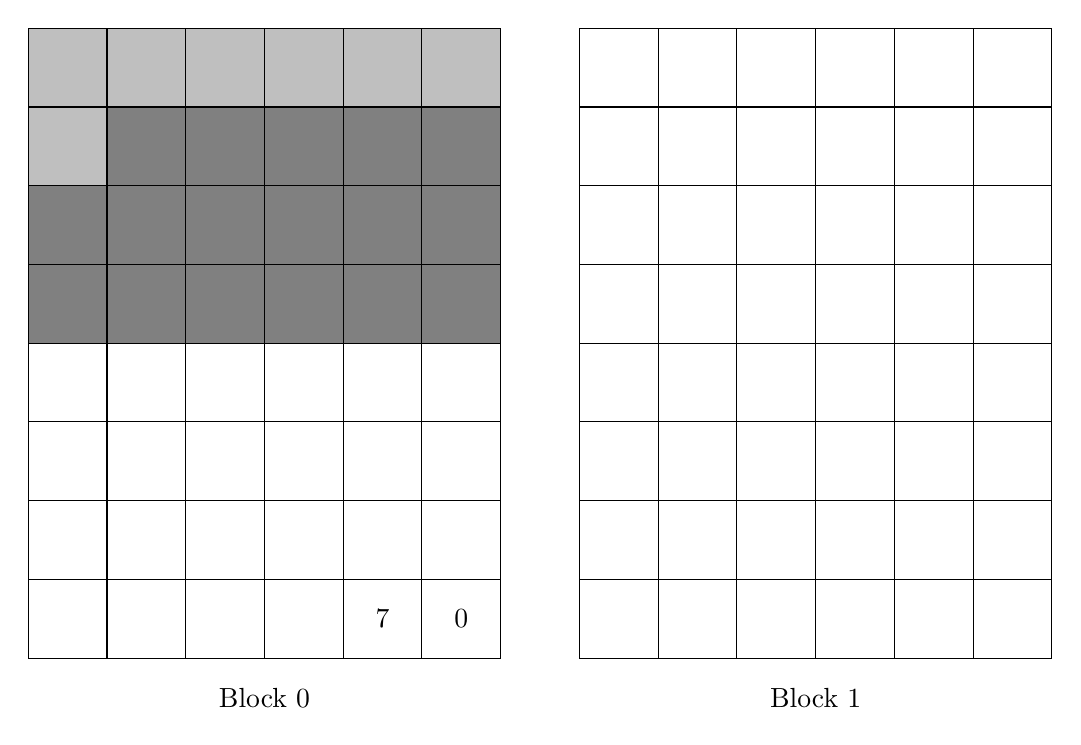
\begin{tikzpicture}
		% Sätze
		\fill[fill=lightgray] (0,8) rectangle +(6,-2);
		\fill[fill=gray] (1,7) rectangle +(5,-1) (0,6) rectangle +(6,-2);

		% Index
		\node at (4.5,0.5) {7};
		\node at (5.5,0.5) {0};

		% Gitter
		\draw (0,0) grid +(6,8) (7,0) grid +(6,8);
		\node at (3,-0.5) {Block~0};
		\node at (10,-0.5) {Block~1};
	\end{tikzpicture}
	\end{center}

	\begin{solution}
	\begin{center}
	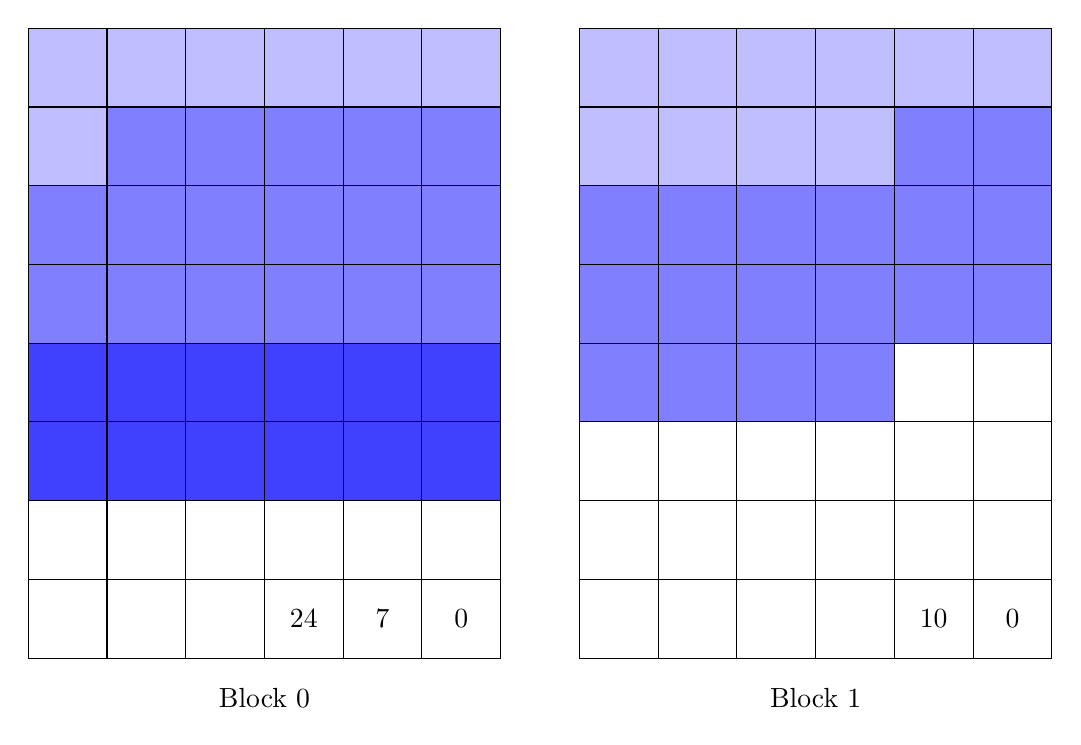
\begin{tikzpicture}
		% Sätze Block 0
		\fill[fill=blue!25] (0,8) rectangle +(6,-2);
		\fill[fill=blue!50] (1,7) rectangle +(5,-1) (0,6) rectangle +(6,-2);
		\fill[fill=blue!75] (0,4) rectangle +(6,-2);

		% Sätze Block 1
		\fill[fill=blue!25] (7,8) rectangle +(6,-1) (7, 7) rectangle +(4, -1);
		\fill[fill=blue!50] (11,7) rectangle +(2,-1) (7,6) rectangle +(6,-2) (7, 4) rectangle +(4, -1);

		% Index Block 0
		\node at (3.5,0.5) {24};
		\node at (4.5,0.5) {7};
		\node at (5.5,0.5) {0};

		% Index Block 1
		\node at (12.5,0.5) {0};
		\node at (11.5,0.5) {10};

		% Gitter
		\draw (0,0) grid +(6,8) (7,0) grid +(6,8);
		\node at (3,-0.5) {Block~0};
		\node at (10,-0.5) {Block~1};
	\end{tikzpicture}
	\end{center}
	12: TID(0, 2), 10: TID(1, 0), 18: TID(1, 1)
	\end{solution}

\begin{beamerText}
\pagebreak
\begin{itemize}
	\item Größe eines Indexeintrags 1~Byte
	\item Größe einer TID 2~Byte
	\end{itemize}
\end{beamerText}

	\item \label{TIDVerlaengerung} Betrachten Sie die folgende Skizze: Block~0 hat zusätzlich zur obigen Ausgangssituation den Satz TID(0, 2) mit der Länge 16 bekommen. Block~1 enthält Satz TID(1, 0) mit der Länge 8.

	Satz TID(0, 0) soll auf die Länge 12 und anschließend Satz TID(0, 1) auf die Länge 23 vergrößert  werden. Zeichnen Sie jeweils die nach den Verlängerungen entstehenden Situationen und geben Sie wieder die zugehörigen TIDs an.

	\begin{center}
	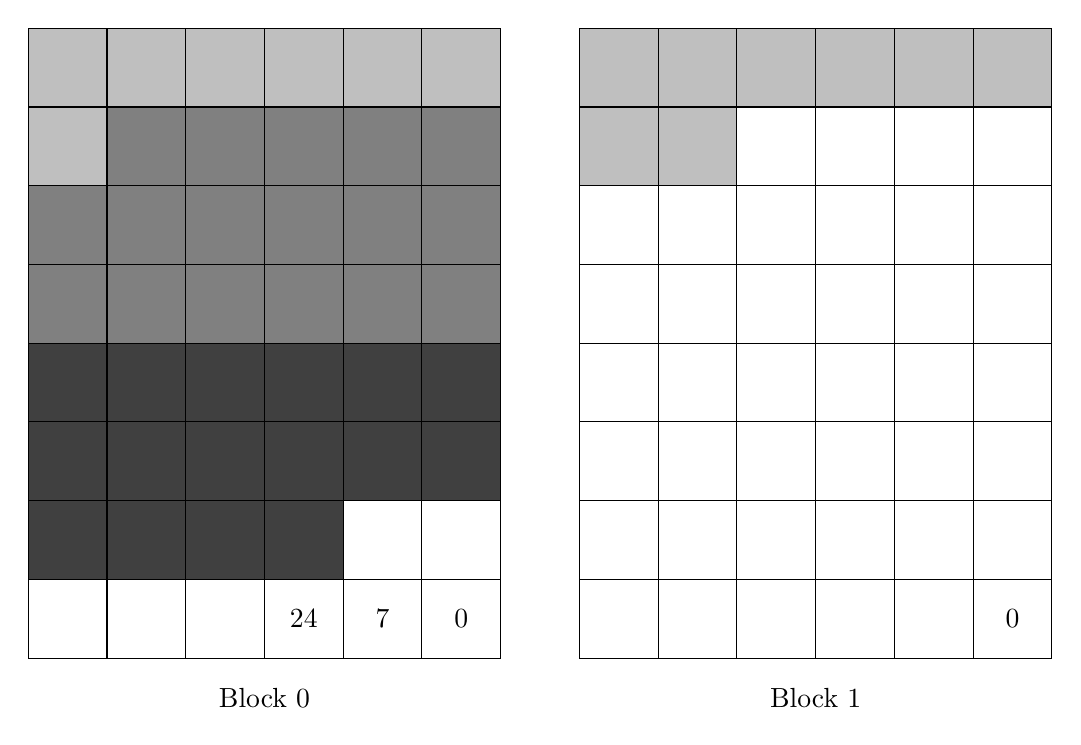
\begin{tikzpicture}
		% Sätze Block 0
		\fill[fill=lightgray] (0,8) rectangle +(6,-2);
		\fill[fill=gray] (1,7) rectangle +(5,-1) (0,6) rectangle +(6,-2);
		\fill[fill=darkgray] (0,4) rectangle +(6,-2) (0,2) rectangle +(4,-1);

		% Sätze Block 1
		\fill[fill=lightgray] (7,8) rectangle +(6,-1) (7,7) rectangle +(2,-1);

		% Index Block 0
		\node at (3.5,0.5) {24};
		\node at (4.5,0.5) {7};
		\node at (5.5,0.5) {0};

		% Index Block 1
		\node at (12.5,0.5) {0};

		% Gitter
		\draw (0,0) grid +(6,8) (7,0) grid +(6,8);
		\node at (3,-0.5) {Block~0};
		\node at (10,-0.5) {Block~1};
	\end{tikzpicture}
	\end{center}

	\begin{solution}
	Verlängerung von TID(0, 0) auf 12: Block 0 ist komplett gefüllt.
	\begin{center}
	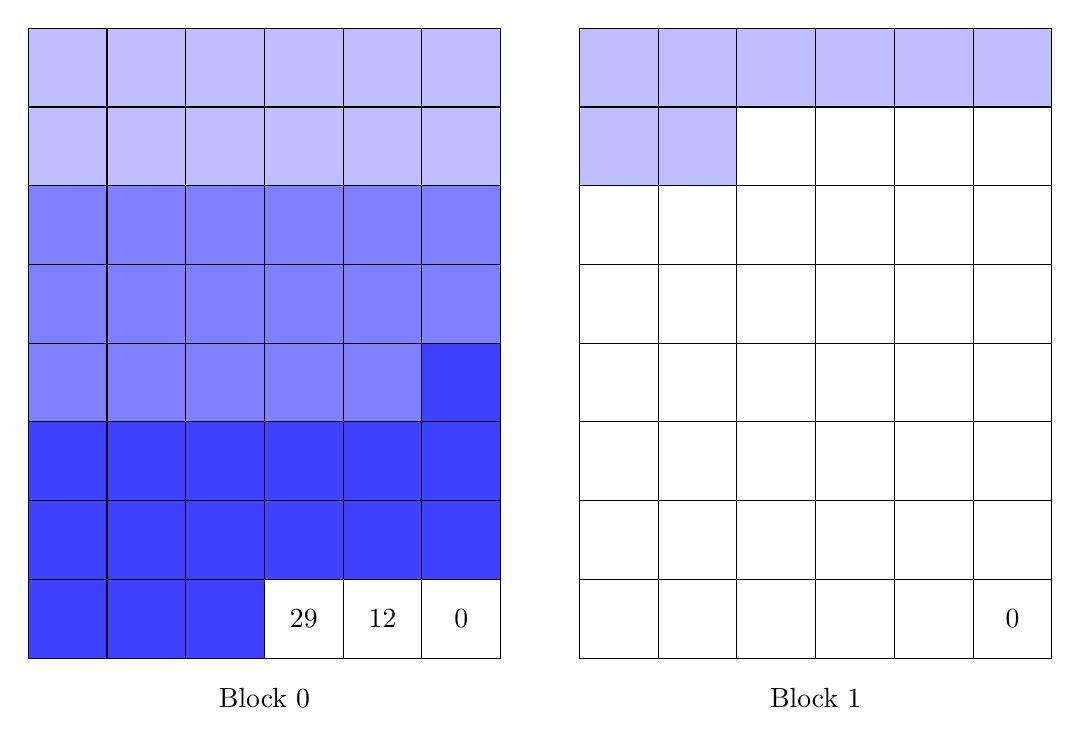
\begin{tikzpicture}
		% Sätze Block 0
		\fill[fill=blue!25] (0,8) rectangle +(6,-2);
		\fill[fill=blue!50] (0,6) rectangle +(6,-3);
		\fill[fill=blue!75] (5,4) rectangle +(1,-1) (0, 3) rectangle +(6, -2) (0, 1) rectangle (3, 0);

		% Sätze Block 1
		\fill[fill=blue!25] (7,8) rectangle +(6,-1) (7, 7) rectangle +(2, -1);

		% Index Block 0
		\node at (3.5,0.5) {29};
		\node at (4.5,0.5) {12};
		\node at (5.5,0.5) {0};

		% Index Block 1
		\node at (12.5,0.5) {0};

		% Gitter
		\draw (0,0) grid +(6,8) (7,0) grid +(6,8);
		\node at (3,-0.5) {Block~0};
		\node at (10,-0.5) {Block~1};
	\end{tikzpicture}
	\end{center}

	7 $\rightarrow$ 12: TID(0, 0), 17: TID(0, 1), 16: TID(0, 2)

	Verlängerung von TID(0, 1) auf 23: Freispeicherverwaltung signalisiert, dass Block~0 komplett gefüllt ist $\Rightarrow$ Überlaufsatz
	\begin{center}
	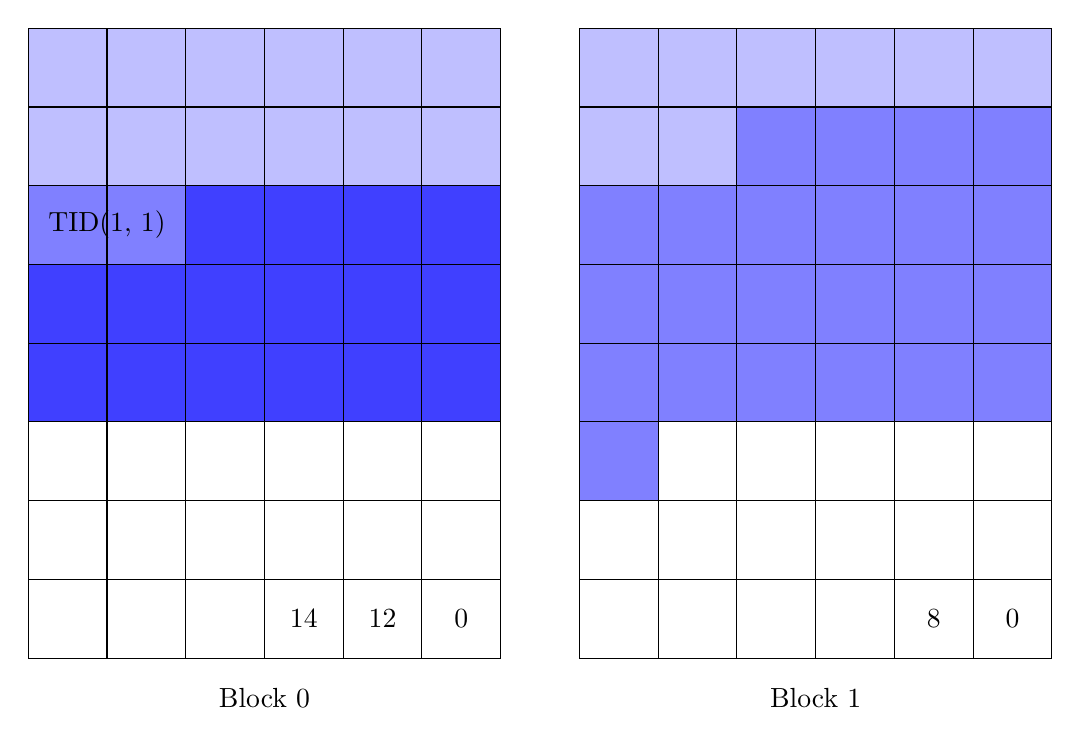
\begin{tikzpicture}
		% Sätze Block 0
		\fill[fill=blue!25] (0,8) rectangle +(6,-2);
		\fill[fill=blue!50] (0,6) rectangle +(2,-1);
		\fill[fill=blue!75] (2,6) rectangle +(4,-1) (0, 5) rectangle +(6, -2);

		% Sätze Block 1
		\fill[fill=blue!25] (7,8) rectangle +(6,-1) (7, 7) rectangle +(2, -1);
		\fill[fill=blue!50] (9,7) rectangle +(4,-1) (7, 6) rectangle +(6, -3) (7, 3) rectangle +(1, -1);

		% Index Block 0
		\node at (3.5,0.5) {14};
		\node at (4.5,0.5) {12};
		\node at (5.5,0.5) {0};

		% Index Block 1
		\node at (1,5.5) {TID(1, 1)};
		\node at (11.5,0.5) {8};
		\node at (12.5,0.5) {0};

		% Gitter
		\draw (0,0) grid +(6,8) (7,0) grid +(6,8);
		\node at (3,-0.5) {Block~0};
		\node at (10,-0.5) {Block~1};
	\end{tikzpicture}
	\end{center}

	12: TID(0, 0), 17 $\rightarrow$ 23: TID(0, 1), 16: TID(0, 2)

	Hinweis: Es ist vermutlich implementierungsabhängig, ob Block~0 gleich reorganisiert wird, d.h. ob TID(0, 2) nach vorne geschoben wird.
	\end{solution}
\begin{beamerText}
\pagebreak
\begin{itemize}
	\item Größe eines Indexeintrags 1~Byte
	\item Größe einer TID 2~Byte
	\end{itemize}
\end{beamerText}

	\item \label{TID_Fragment} Nach den beiden Satzvergrößerungen aus Teilaufgabe \ref{TIDVerlaengerung}) soll noch ein Satz der Länge 57 eingefügt werden. Zeichnen Sie die entstehende Situation und geben Sie die zugehörige TID des Satzes an. Gehen Sie davon aus, dass in Block~2 noch keine Sätze abgelegt sind.

\begin{normalText}
	Wenn ein einzufügender Satz die maximale Blockgröße überschreitet, muss er fragmentiert werden. Fragmente sind normalerweise so groß wie der maximal nutzbare Speicher eines Blocks, nur das letzte Fragment eines Satzes darf kleiner sein. Das bedeutet, die Fragmente eines Satzes haben alle die maximal nutzbare Speichergröße und werden jeweils in neue, unbefüllte Blöcke abgelegt, nur das letzte Fragment kann, falls es einen bereits teilweise gefüllten Block mit ausreichend freiem Speicher gibt, in diesem abgelegt werden. Der Zugriff auf einen solchen Satz erfolgt transparent, d.\,h. die Fragmente sind nach außen hin nicht sichtbar.

	Legen Sie in dieser Teilaufgabe zusätzlich zu den bisher in den Blöcken abgelegten Informationen einen Fragmentierungs-Header der Größe 2~Byte vor den Fragmenten eines Satzes mit ab. Dieser zeigt auf das nächste Fragment des Satzes. Wird auch vor dem letzten Fragment ein Fragmentierungs-Header benötigt?
\end{normalText}

	\begin{center}
	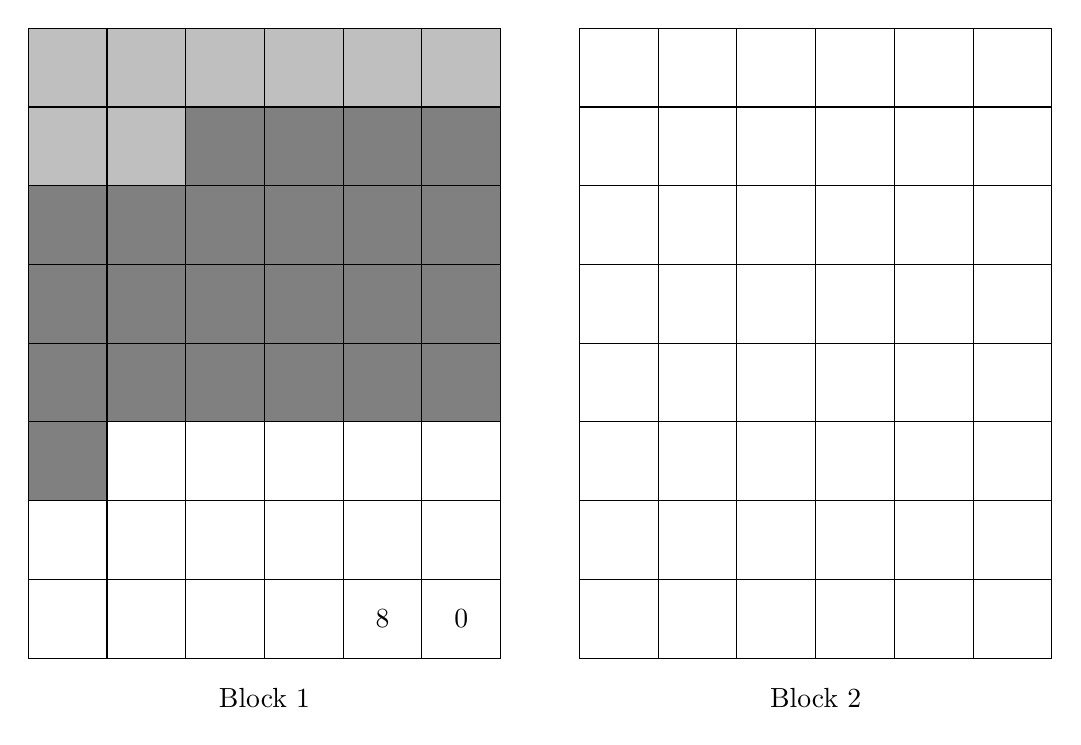
\begin{tikzpicture}
		% Sätze Block 1
		\fill[fill=lightgray] (0,8) rectangle +(6,-2);
		\fill[fill=gray] (2,7) rectangle +(4,-1) (0,6) rectangle +(6,-3) (0,3) rectangle +(1,-1);

		% Index Block 1
		\node at (5.5,0.5) {0};
		\node at (4.5,0.5) {8};
		% Gitter
		\draw (0,0) grid +(6,8) (7,0) grid +(6,8);
		\node at (3,-0.5) {Block~1};
		\node at (10,-0.5) {Block~2};
	\end{tikzpicture}
	\end{center}

\begin{beamerText}
	\pagebreak
	Wenn ein einzufügender Satz die maximale Blockgröße überschreitet, muss er fragmentiert werden. Fragmente sind normalerweise so groß wie der maximal nutzbare Speicher eines Blocks, nur das letzte Fragment eines Satzes darf kleiner sein. Das bedeutet, die Fragmente eines Satzes haben alle die maximal nutzbare Speichergröße und werden jeweils in neue, unbefüllte Blöcke abgelegt, nur das letzte Fragment kann, falls es einen bereits teilweise gefüllten Block mit ausreichend freiem Speicher gibt, in diesem abgelegt werden. Der Zugriff auf einen solchen Satz erfolgt transparent, d.\,h. die Fragmente sind nach außen hin nicht sichtbar.

	Legen Sie in dieser Teilaufgabe zusätzlich zu den bisher in den Blöcken abgelegten Informationen einen Fragmentierungs-Header der Größe 2~Byte vor den Fragmenten eines Satzes mit ab. Dieser zeigt auf das nächste Fragment des Satzes. Wird auch vor dem letzten Fragment ein Fragmentierungs-Header benötigt?
\end{beamerText}

	\begin{solution}
	Das letzte Fragment benötigt keinen Fragmentierungs-Header, da ja kein weiteres Fragment mehr kommt.

	Fragmentiere Satz der Länge 57 in 2 Fragmente der Größe 45 (= Blockgröße – 1~Byte Indexeintrag – 2~Byte Fragmentierungs-Header) und 12 (= Rest). Lege Fragment der Größe 45 in neuen Block 2. Fragment der Größe 12 passt noch in Block 1.
	\begin{center}
	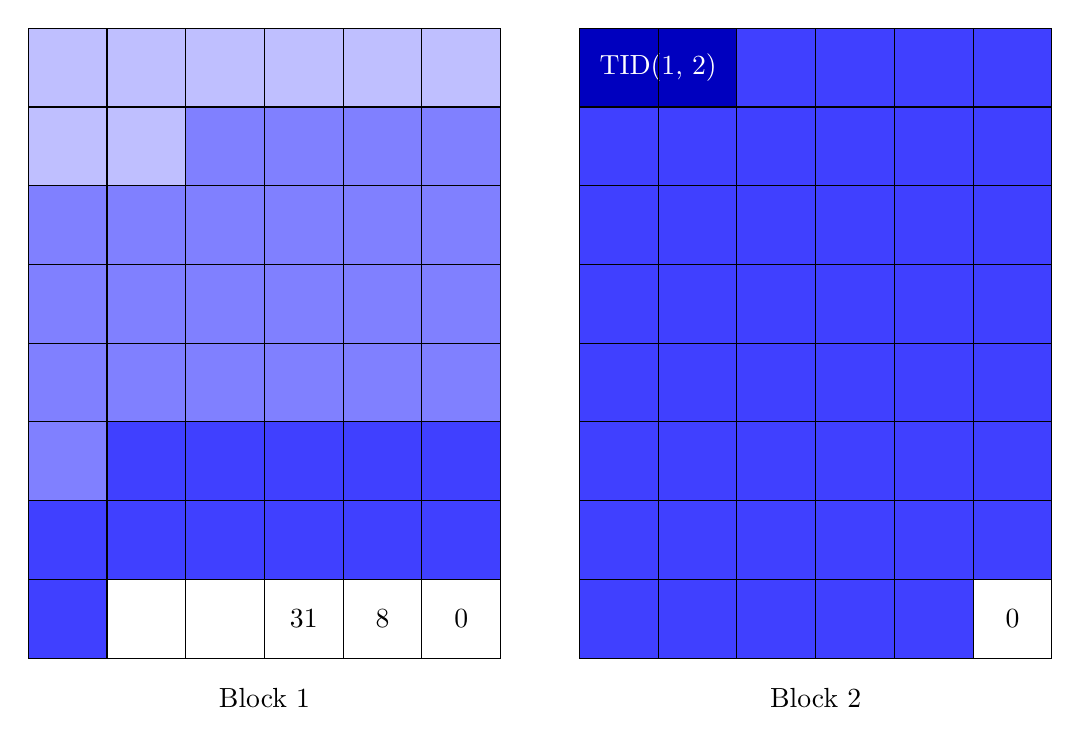
\begin{tikzpicture}
		% Sätze Block 1
		\fill[fill=blue!25] (0,8) rectangle +(6,-2);
		\fill[fill=blue!50] (2,7) rectangle +(4,-1) (0,6) rectangle +(6,-3) (0,3) rectangle +(1,-1);
		\fill[fill=blue!75] (1, 3) rectangle +(5, -1) (0, 2) rectangle +(6, -1) (0, 1) rectangle +(1, -1);
		% Index Block 1
		\node at (5.5,0.5) {0};
		\node at (4.5,0.5) {8};
		\node at (3.5, 0.5) {31};

		%Sätze Block 2
		\fill[fill=blue!75!black] (7, 8) rectangle +(2, -1);
		\fill[fill=blue!75] (9,8) rectangle +(4, -1) (7, 7) rectangle +(6, -6) (7, 1) rectangle +(5, -1);

		%Index Block 2
		\node at (12.5, 0.5) {0};
		\node at (8,7.5) {\color{white}TID(1, 2)};

		% Gitter
		\draw (0,0) grid +(6,8) (7,0) grid +(6,8);
		\node at (3,-0.5) {Block~1};
		\node at (10,-0.5) {Block~2};
	\end{tikzpicture}
	\end{center}

	57: TID(2, 0)

	Wichtig ist die Erkenntnis, dass der Zeiger von einem Fragment auf das nächste oder von der ursprünglichen Satzposition auf die tatsächliche wieder eine TID ist.
	\end{solution}

	\item \label{TID_erw_red} Betrachten \selbst Sie die aus Teilaufgabe \ref{TID_Fragment}) resultierende Situation.
	Erweitern Sie nun den Satz mit TID(0,1) auf die Länge 26.
	Verkleinern Sie anschließend den Satz mit TID(2,0) auf die Länge 10.

	\begin{note}
		Für die Umstrukturierung des Satzes mit TID(0,1) benötigen wir zunächst die Blöcke 0 und 1.

		Ausgangssituation

		\begin{center}
			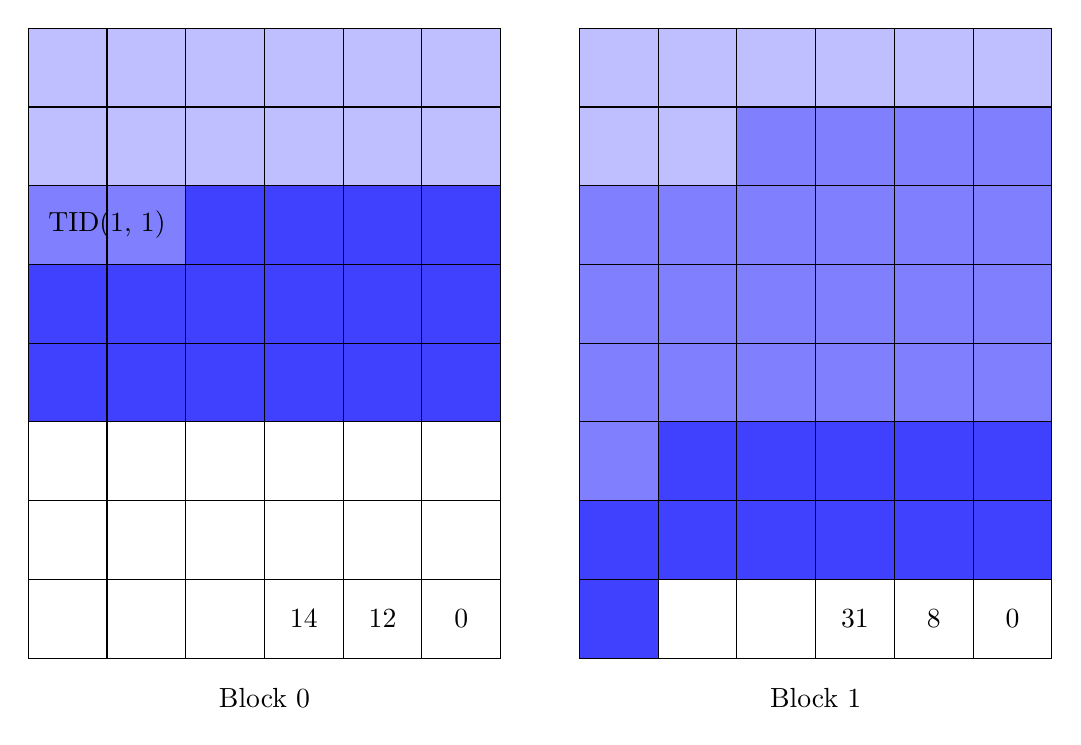
\begin{tikzpicture}
				% Sätze Block 0
				\fill[fill=blue!25] (0,8) rectangle +(6,-2);
				\fill[fill=blue!50] (0,6) rectangle +(2,-1);
				\fill[fill=blue!75] (2,6) rectangle +(4,-1) (0, 5) rectangle +(6, -2);

				% Sätze Block 1


				\fill[fill=blue!25] (7,8) rectangle +(6,-2);
				\fill[fill=blue!50] (9,7) rectangle +(4,-1) (7,6) rectangle +(6,-3) (7,3) rectangle +(1,-1);
				\fill[fill=blue!75] (8, 3) rectangle +(5, -1) (7, 2) rectangle +(6, -1) (7, 1) rectangle +(1, -1);
				% Index Block 0
				\node at (3.5,0.5) {14};
				\node at (4.5,0.5) {12};
				\node at (5.5,0.5) {0};

				% Index Block 1
				\node at (1,5.5) {TID(1, 1)};
				\node at (10.5,0.5) {31};
				\node at (11.5,0.5) {8};
				\node at (12.5,0.5) {0};
				% Gitter
				\draw (0,0) grid +(6,8) (7,0) grid +(6,8);
				\node at (3,-0.5) {Block~0};
				\node at (10,-0.5) {Block~1};
			\end{tikzpicture}
		\end{center}
		Bei der Verlängerung von TID(0,1) signalisiert die Freispeicherverwaltung, dass Block 1 zu klein ist $\Rightarrow$ Überlaufsatz.

		Hinweis: Es ist vermutlich implementierungsabhängig, ob Block~1 gleich reorganisiert wird, d.h. ob TID(1, 2) nach vorne geschoben wird.

		Situation nach dem Verlängern:

		\begin{center}
			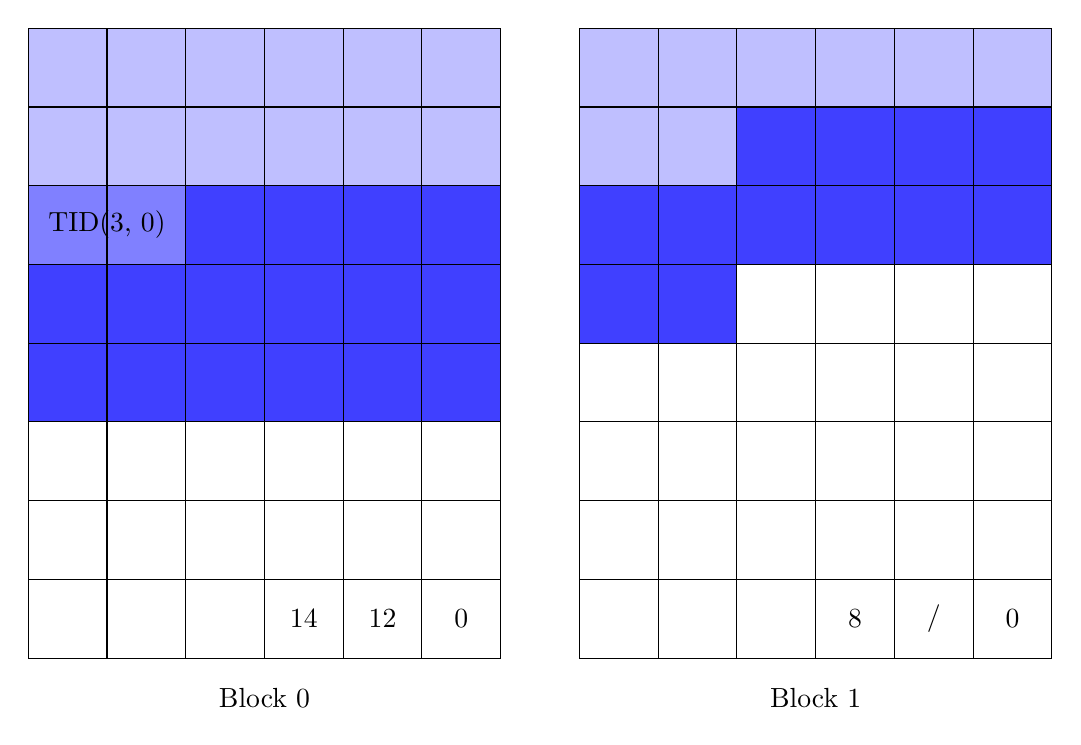
\begin{tikzpicture}
			% Sätze Block 0
			\fill[fill=blue!25] (0,8) rectangle +(6,-2);
			\fill[fill=blue!50] (0,6) rectangle +(2,-1);
			\fill[fill=blue!75] (2,6) rectangle +(4,-1) (0, 5) rectangle +(6, -2);

			% Sätze Block 1

			\fill[fill=blue!25] (7,8) rectangle +(6,-2);

			\fill[fill=blue!75] (9, 7) rectangle +(4, -1) (7, 6) rectangle +(6, -1) (7, 5) rectangle +(2, -1);
			% Index Block 0
			\node at (3.5,0.5) {14};
			\node at (4.5,0.5) {12};
			\node at (5.5,0.5) {0};

			% Index Block 1
			\node at (1,5.5) {TID(3, 0)};
			\node at (10.5,0.5) {8};
			\node at (11.5,0.5) {/};
			\node at (12.5,0.5) {0};
			% Gitter
			\draw (0,0) grid +(6,8) (7,0) grid +(6,8);
			\node at (3,-0.5) {Block~0};
			\node at (10,-0.5) {Block~1};
			\end{tikzpicture}
		\end{center}
		\begin{center}
			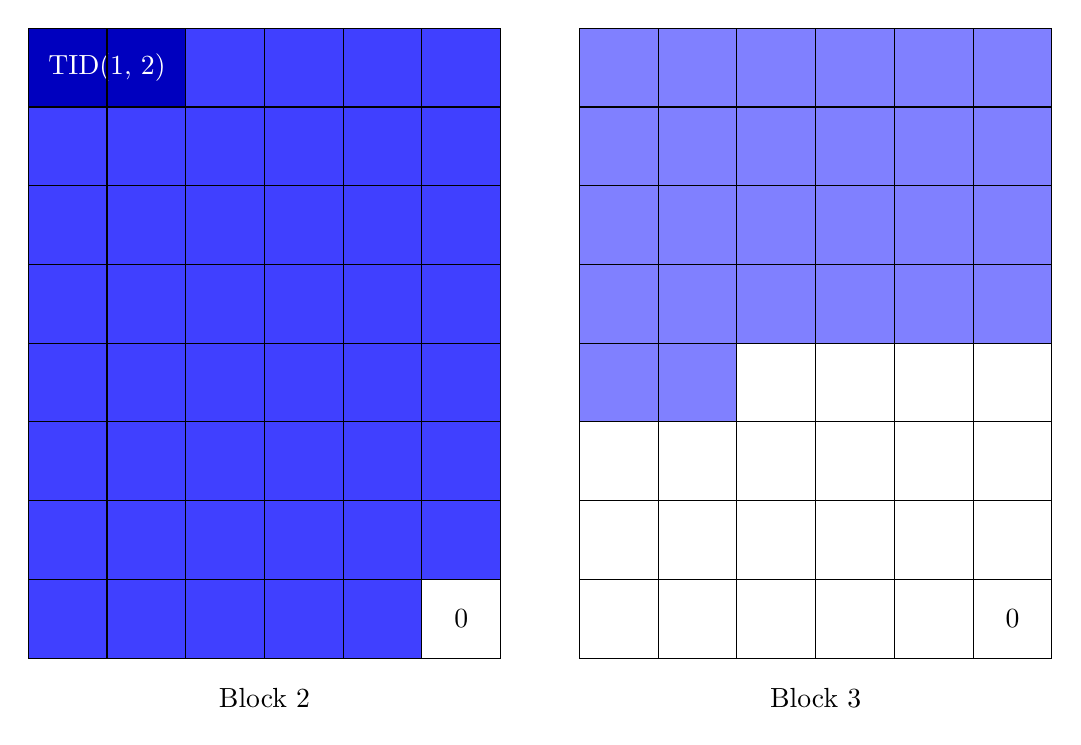
\begin{tikzpicture}
			%Sätze Block 2
			\fill[fill=blue!75!black] (0, 8) rectangle +(2, -1);
			\fill[fill=blue!75] (2,8) rectangle +(4, -1) (0, 7) rectangle +(6, -6) (0, 1) rectangle +(5, -1);

			%Sätze Block 3
			\fill[fill=blue!50] (7,8) rectangle +(6,-4) (7,4) rectangle +(2,-1);

			%Index Block 2
			\node at (5.5, 0.5) {0};
			\node at (1,7.5) {\color{white}TID(1, 2)};

			%Index Block 3
			\node at (12.5, 0.5) {0};
			% Gitter
			\draw (0,0) grid +(6,8) (7,0) grid +(6,8);
			\node at (3,-0.5) {Block~2};
			\node at (10,-0.5) {Block~3};

			\end{tikzpicture}
		\end{center}

		Wichtige ist hierbei, dass der Eintrag in TID(0,2) auf (3,0) umgebogen wird und TID(1,1) als ungültig markiert wird.

		Als Optimierung könnte zwischen ursprünglich nach außen sichtbaren gelöschten Sätzen und entfernten Überlaufsätzen unterschieden werden.
		Wenn deren Indexeinträge unterschiedlich als ungültig markiert werden, können TIDs von Überlaufsätzen, die nie nach außen gegeben wurden, wiederverwendet werden, was Indexeinträge spart.

		Für die Verkleinerung von TID(2,0) auf die Länge 10 verändern sich nun die Blöcke 1 und 2.

		Situation nach dem Verkleinern:

		\begin{center}
			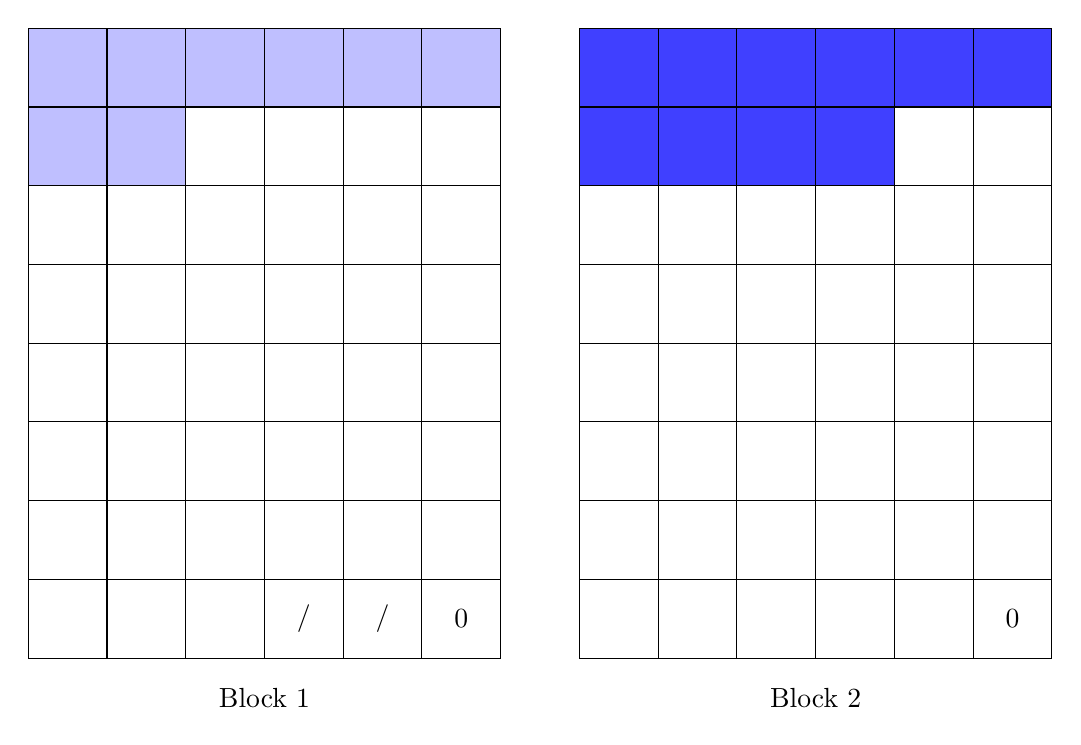
\begin{tikzpicture}
			% Sätze Block 1
			\fill[fill=blue!25] (0,8) rectangle +(6,-1) (0,7) rectangle +(2,-1);

			% Index Block 1
			\node at (5.5,0.5) {0};
			\node at (4.5,0.5) {/};
			\node at (3.5,0.5) {/};


			%Sätze Block 2

			\fill[fill=blue!75] (7,8) rectangle +(6, -1) (7, 7) rectangle +(4, -1);

			%Index Block 2
			\node at (12.5, 0.5) {0};

			% Gitter
			\draw (0,0) grid +(6,8) (7,0) grid +(6,8);
			\node at (3,-0.5) {Block~1};
			\node at (10,-0.5) {Block~2};
			\end{tikzpicture}
		\end{center}
	\end{note}
\end{enumerate}

